\section{Metode}
\noindent\textbf{Utstyr}:
\begin{itemize}
    \item Telefon
    \item Telefonholder
    \item Trefot
    \item Vater
\end{itemize}
  
For målingene ble en trefot brukt for å stabilisere telefonen og sørge for minst mulig bevegelse som kunne påvirke resultatene. Et vater siktet først inn på Nidarosdomen og telefonen ble lagt ved siden av vateret som figur \ref{fig:med_vater} viser. Før alle målingene ble gjort ble programmet Phypox kalibrert ved å snu rundt på mobilen i rundt 30 sekunder. Det ble så gjort tre målinger med tre forskjellige mobiler. Dette gjentok seg tre ganger.

Så ble vateret siktet inn på tyholttårnet på samme måte som målingene på Nidarosdomen ble gjennmført. Denne gangen ble mobilen slåt..
Målingene ble gjort rett utenfor hovedbygningen til NTNU i starten av broen på veien "Øvre Alle" slik at det var både mulig å se toppen av Nidarosdomen og tyholttårnet på samme sted.  

\begin{figure}
    \centering
    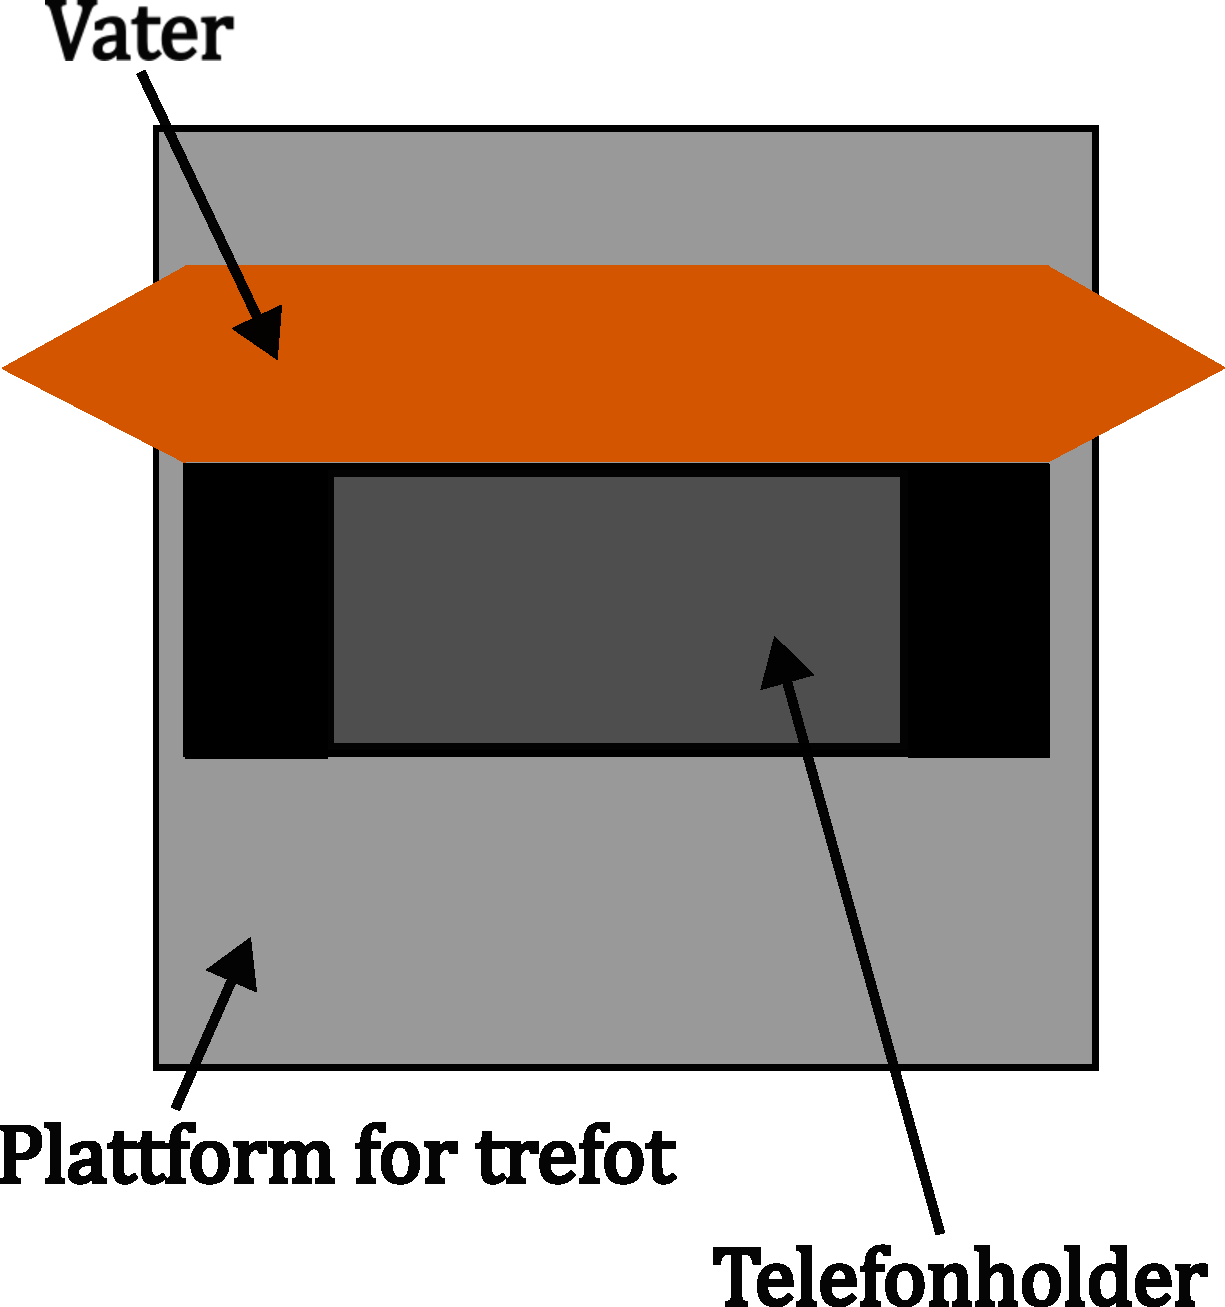
\includegraphics[width=0.55\textwidth]{img/Plattform med vater.pdf}
    \caption{Figuren viser oppsettet under målingene. Et vater ble brukt for å sikte inn på Nidarosdomen og Tyholttårnet og viste i hvilken retning mobilen skulle ligge. 
        }
    \label{fig:med_vater}
\end{figure}